\documentclass{beamer} % [aspectratio=169]
\usetheme{ucl}
\setbeamercolor{banner}{bg=brightblue}
\setbeamersize{description width=2em}
\setbeamertemplate{navigation symbols}{\vspace{-2ex}} 

%\usepackage{fontspec}
\usepackage[utf8]{inputenc}
% \usepackage[english, greek]{babel}


\usepackage[T1]{fontenc} % Turn £ into $
\usepackage{minted}
\usemintedstyle{emacs}

\usepackage{fancyvrb}
\usepackage{xcolor}
\usepackage{url}

\usepackage{natbib}
\usepackage{bibentry}
\usepackage{url}


\usepackage{tikz}
\usetikzlibrary{positioning}



\newcommand\emc[1]{\textcolor{brightblue}{\textbf{#1}}}

\AtBeginSection[]{
  \begin{frame}
  \vfill
  \centering
  \begin{beamercolorbox}[sep=8pt,center,shadow=true,rounded=true]{title}
    \usebeamerfont{title}\insertsectionhead\par%
  \end{beamercolorbox}
  \vfill
  \end{frame}
}

\author{Prof.\ George Danezis, University College London, UK}
\title{About this module.}
\subtitle{ENGS102P: Design and Professional Skills }
% \institute{}
\date{Term 1, 2017}


\begin{document}
\nobibliography*


\frame{
\titlepage
}


\begin{frame}
\frametitle{Welcome to UCL Engineering \& Computer Science!}

Our aim is to prepare you to be the \emc{best engineers in the world}!

\vspace{10mm}
Engineering is the discipline of \emc{shaping the world} around us 

for the \emc{benefit of humanity}.

\vspace{5mm}
\centering

\includegraphics[height=20mm]{img/internet.jpg} \quad
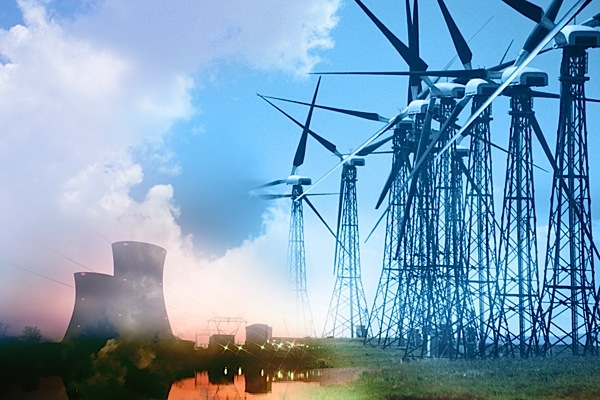
\includegraphics[height=20mm]{img/power.jpg} \quad
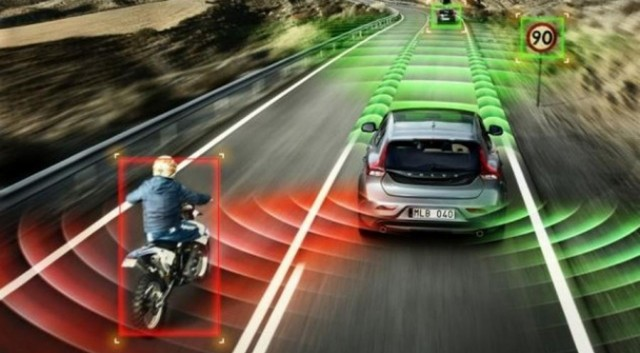
\includegraphics[height=20mm]{img/cars.jpg}

\end{frame}

\begin{frame}
\frametitle{The cost of bad engineering.}

Never forget the \emc{human cost} of bad engineering, 

and your \emc{personal professionals responsibility}.

\vspace{10mm}
\centering
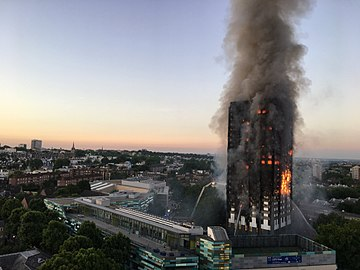
\includegraphics[height=23mm]{img/Grenfell.jpg} \quad
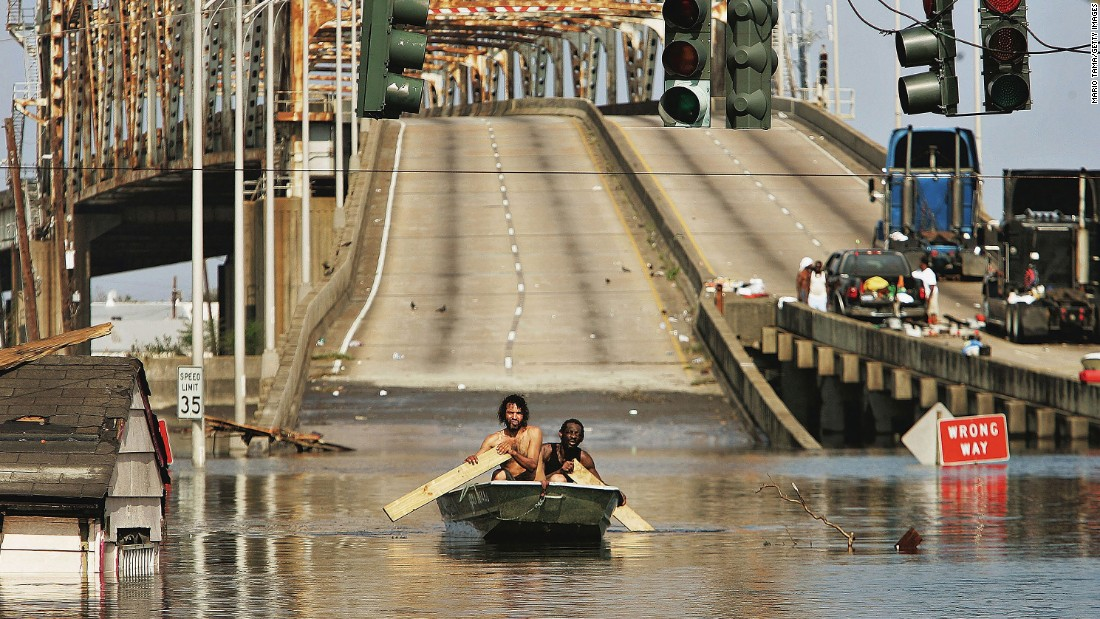
\includegraphics[height=23mm]{img/katrina.jpg} \quad
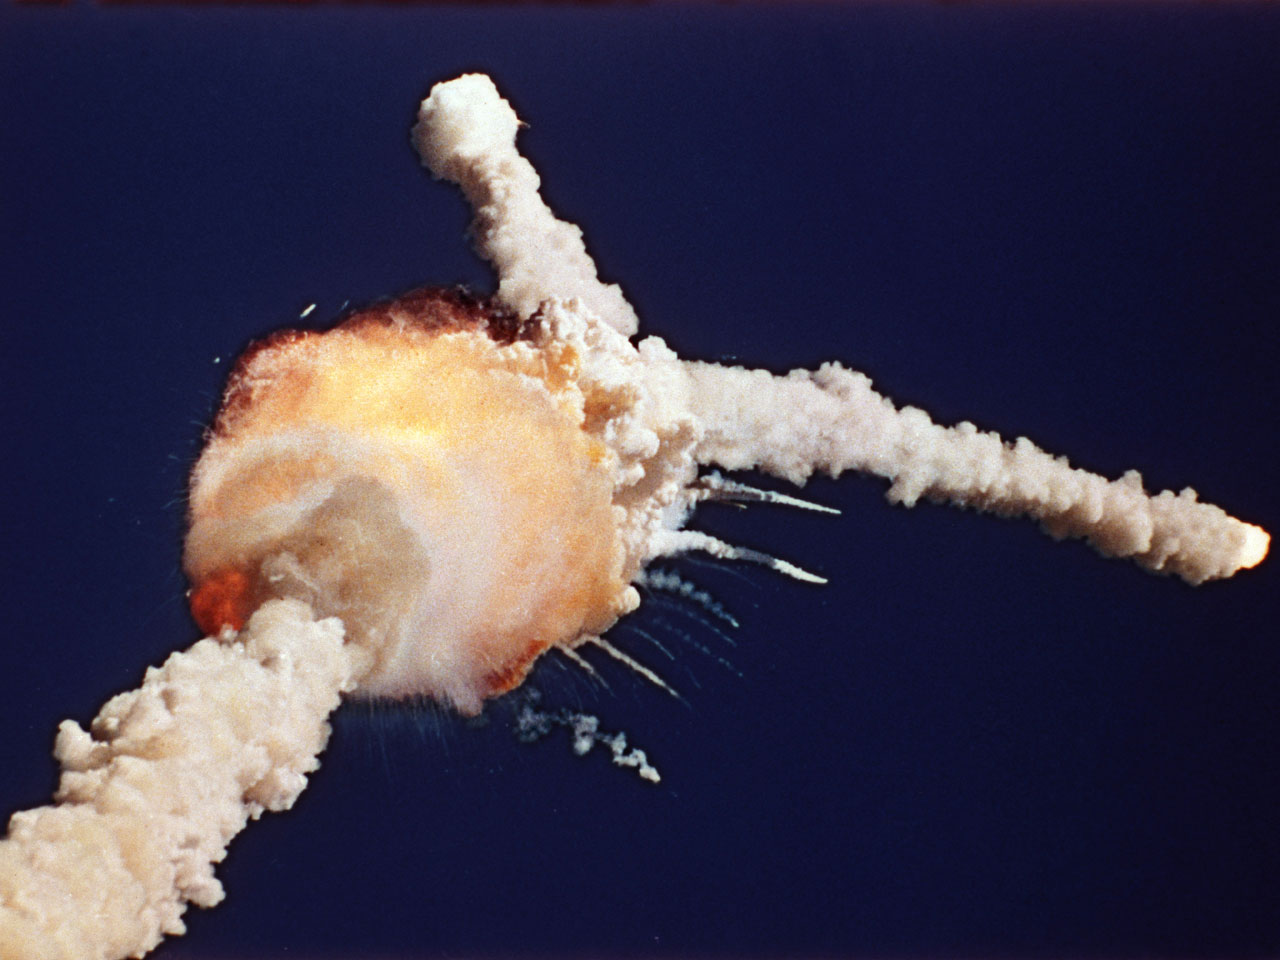
\includegraphics[height=23mm]{img/challenger.jpg}

\end{frame}

\begin{frame}
\frametitle{Overall aims of the ENGS102P.} 

The essence of good engineering is \emc{quality}. This course aims to:

\begin{itemize}
	\item Teach you professional skills important in all engineering.
	\item Teach you computer science specific professional skills.
	\item Expose you to important social and ethical discussions.
	\item Provide opportunities to practice all those skills.
\end{itemize}

\vspace{3mm}
Term 1 teaching is delivered jointly by faculty lecturers and department lecturers. Term 2 is delivered by the department and devoted to software engineering scenarios to support Term 1 concepts.

\end{frame}

\begin{frame}
\frametitle{Who are we?} 

\begin{description}
\item[George Danezis (me)] is a Professor of Security and Privacy Engineering at UCL, with interests in anonymity, privacy, distributed Systems and decentralization.
\item[Stefano Vissicchio] is a Lecturer at UCL, with interests in in theory, algorithms and systems for efficiently and reliably managing communication networks.
\item[Matteo Sammartino] is a Researcher at UCL with interests in formal languages, coalgebras, process calculi, and automata learning.
\item[Kate Roach] is a Senior Teaching Fellow, writer and a researcher with a special interest in the influence of technology, science or engineering on people and vice versa.
\item[Sunny Baines] is a Teaching Fellow, with backgrounds in both technology and journalism, and is a specialist in teaching engineers to communicate.
\end{description}

\end{frame}

\begin{frame}
\frametitle{What Engineering Skills?} 

You will spend a significant part of your career \emc{communicating} with other engineers, other professionals and the public.

\vspace{3mm}
To help you we teach:
\begin{itemize}
\item Technical writing \& Technical argument.
\item Engineering visualization.
\item Technical Presentations.
\item Effective team work \& dynamics.
\end{itemize}

\vspace{3mm}
Those are supported with a number of courseworks, feedback \& peer assessment across disciplines.

\end{frame}


\begin{frame}
\frametitle{What Computer Science \& Software Engineering Skills?} 

Computer Science lies at the intersection of \emc{mathematics} and \emc{engineering}. It solves problems through the manipulation of \emc{information}, and \emc{computation}.

\vspace{3mm}
This module will cover:
\begin{itemize}
	\item The \emc{principles of programming} illustrated in Python.
	\item The principles of \emc{algorithms}, their implementation, cost and correctness.
	\item The tools and techniques to ensure \emc{quality software}.
	\item The organization of \emc{software production} in teams.
	\item Key tools and technologies for \emc{rapid prototyping}.
	\item Important \emc{social and ethical} dimensions of the information society.
\end{itemize}

\end{frame}

\begin{frame}
\frametitle{Key times, dates and locations} 

The \emc{rooms change every week!}
Familiarize your self with the timetable: \url{https://timetable.ucl.ac.uk}.

\begin{itemize}
	\item Tuesday 09:00--11:00 -- Lectures.
	\item Friday 11:00--13:00 -- Lectures.
\end{itemize}

\vspace{3mm}
Computer Science specific assessments due dates \\ (individual programming exercises):
\begin{itemize}
	\item 1 November -- Peer-reviewed exercise.
	\item 29 November -- Assessed exercise.
	\item 10 January -- Assessed exercise.
\end{itemize}
We will provide more information and submission during term.


\end{frame}

\begin{frame}
\frametitle{Course material.} 

All course material is available on-line, on github and moodle.

\vspace{10mm}
Computer Science specific syllabus, slides \& code: 

\url{https://github.com/gdanezis/Design_and_Professional_Skills}



\end{frame}

% ---------------------------------

\bibliographystyle{alpha}
\nobibliography{references}

\end{document}